\documentclass[twoside]{article}
\usepackage{amsmath}
\usepackage{amssymb}
\usepackage{algorithm}  
\usepackage{algorithmicx}  
\usepackage{algpseudocode}  
\usepackage{amsmath}
\usepackage{bbm}  

  
\renewcommand{\algorithmicrequire}{\textbf{Input:}}  
\renewcommand{\algorithmicensure}{\textbf{Output:}} 
\DeclareMathOperator*{\argmax}{arg\,max}
\usepackage{epsfig} 
\usepackage{graphicx}
\usepackage{subfigure}

\setlength{\oddsidemargin}{0.25 in}
\setlength{\evensidemargin}{-0.25 in}
\setlength{\topmargin}{-0.6 in}
\setlength{\textwidth}{6.5 in}
\setlength{\textheight}{8.5 in}
\setlength{\headsep}{0.75 in}
\setlength{\parindent}{0 in}
\setlength{\parskip}{0.1 in}

\newcommand{\lecture}[3]{
   \pagestyle{myheadings} 
   \thispagestyle{plain}
   \newpage
   \setcounter{page}{1}
   \noindent
   \begin{center}
   \framebox{
      \vbox{\vspace{2mm}
    \hbox to 6.28in { {\bf 10-707: Deep Learning, Fall 2017 \hfill} }
       \vspace{6mm}
       \hbox to 6.28in { {\Large \hfill #1  \hfill} }
       \vspace{6mm}
       \hbox to 6.28in { {\it Lecturer: #2 \hfill Name: #3} }
      \vspace{2mm}}
   }
   \end{center}
   \markboth{#1}{#1}
   \vspace*{4mm}
}

\begin{document}

\lecture{Homework 2}{Russ Salakhutdinov }{Yuan Liu(yuanl4)} % Lecture name, Lecturer, Scribes
\section{Problem 1}
\paragraph{How to compute derivation:}
\begin{itemize}
\item The input image is a 2-D matrix $X$, the size is $d\times d$.
\item Convolutional Layer: the parameter of feature map $i \in \{1,2\}$ is $W^{i}$. They are two 2-D matrixes, the size of each matrix is $k\times k$.\\

The output of the convolutional layer is two 2-D matrixes $Y^{i},i \in \{1,2\}$, the size of each matrix is $\frac{d-k+1}{s}\times \frac{d-k+1}{s}$
$$Y_{m,n}^i = \sum_{p=1}^k \sum_{q=1}^k X_{(m-1)s + p, (n-1)s+q} W_{p,q}^i$$
Then we can get:
$$\frac{\partial Y_{m,n}^i }{\partial W_{p,q}^i} = X_{(m-1)s + p, (n-1)s+q} \eqno{(1)}$$

The derivation input of the convolutional layer is two 2-D matrix $\frac{\partial Loss}{\partial Y^{i}},i \in \{1,2\}$, the size of each matrix is $\frac{d-k+1}{s}\times \frac{d-k+1}{s}$.
Then we can get:
$$\frac{\partial Loss}{\partial W_{p,q}^i} = \sum_{m,n=1}^{\frac{d-k+1}{s}}\frac{\partial Loss}{ \partial Y^i}_{m,n} \frac{\partial Y_{m,n}^i }{\partial W_{p,q}^i}
=\sum_{m,n=1}^{\frac{d-k+1}{s}}\frac{\partial Loss}{ \partial Y^i}_{m,n} X_{(m-1)s + p, (n-1)s+q}$$

\item Pooling Layer: The output of pooling layer is two 2-D matrixes $P^{i},i \in \{1,2\}$, the size of each matrix is $(\frac{d-k+1}{s}-p+1)\times (\frac{d-k+1}{s}-p+1)$.
$$P^{k}_{m,n} = \max_{i,j \in \{1,...,p\}} Y^k_{m+i-1,n+j-1} $$
The derivation input of the pooling layer is two 2-D matrix $\frac{\partial Loss}{\partial P^{i}},i \in \{1,2\}$, the size of each matrix is $(\frac{d-k+1}{s}-p+1)\times (\frac{d-k+1}{s}-p+1)$.
Then we gan get the derivation output is:
$$\frac{\partial P^k_{m,n}}{\partial Y^K_{m+i-1,n+j-1}} = \mathbbm{1}(i,j = \argmax_{i,j}Y^k_{m+i-1,n+j-1}) \eqno{(2)}$$
$$\frac{\partial Loss}{\partial Y^{k}}_{m,n} = \sum_{i,j=1}^p \frac{\partial Loss}{\partial P^k}_{m+i-1, n+j-1} \mathbbm{1}(i,j = \argmax_{i,j \in \{1,...,p\}} Y^k_{m+i-1,n+j-1})$$

\item Flatten Layer, which convert the two 2-dimension matrixes into a vector. The length of this vector is $2(\frac{d-k+1}{s}-p+1)^2$.
%$$F_i = P^{k}_{m , n}$$
%$$k = \lceil \frac{i}{(\frac{d-k+1}{s}-p+1)^2} \rceil$$
%$$m=\lceil \frac{i-(\frac{d-k+1}{s}-p+1)^2(k-1)}{\frac{d-k+1}{s}-p+1}\rceil $$
%$$n = i-(\frac{d-k+1}{s}-p+1)^2(k-1) -(\lceil \frac{i-(\frac{d-k+1}{s}-p+1)^2(k-1)}{\frac{d-k+1}{s}-p+1}\rceil-1)(\frac{d-k+1}{s}-p+1)$$
$$P_{m,n}^k = F_{(k-1)*(\frac{d-k+1}{s}-p+1)^2+(m-1)*(\frac{d-k+1}{s}-p+1)+n}$$
$$\frac{\partial P_{m,n}^k}{\partial F_{i}} = \mathbbm{1}(i=  (k-1)*(\frac{d-k+1}{s}-p+1)^2+(m-1)*(\frac{d-k+1}{s}-p+1)+n) \eqno{(3)}$$
$$\frac{\partial Loss}{\partial P^{k}_{m , n}}=\frac{\partial Loss}{\partial F_{(k-1)*(\frac{d-k+1}{s}-p+1)^2+(m-1)*(\frac{d-k+1}{s}-p+1)+n}}$$

\item Softmax Layer: Assume $k=2(\frac{d-k+1}{s}-p+1)^2$, the output of this softmax layer is a vector $S$, which size is k.
$$S_i = \frac{e^{F_i}}{\sum_{j=1}^k e^{F_j}} $$
The derivation input of the softmax layer is a vector $\frac{\partial Loss}{\partial S}$, which size is k.
$$\frac{\partial S_i}{\partial F_j} = \frac{\frac{e^{F_i}}{\partial F_j} (\sum_{j=1}^k e^{F_j}) - e^{F_i}e^{F_j}}{(\sum_{j=1}^k e^{F_j})^2}
= \frac{\mathbbm{1}(i=j) (\sum_{j=1}^k e^{F_j}) - e^{F_i}e^{F_j}}{(\sum_{j=1}^k e^{F_j})^2}
=\frac{\mathbbm{1}(i=j) }{\sum_{j=1}^k e^{F_j}}-\frac{e^{F_i+F_j}}{(\sum_{j=1}^k e^{F_j})^2}$$
$$\frac{\partial Loss}{\partial F_j}=\sum_{i=1}^k \frac{\partial Loss}{\partial S_i}\frac{\partial S_i}{\partial F_j}=\sum_{i=1}^k \frac{\partial Loss}{\partial S_i}( \frac{\mathbbm{1}(i=j) }{\sum_{j=1}^k e^{F_j}}-\frac{e^{F_i+F_j}}{(\sum_{j=1}^k e^{F_j})^2} )$$
\end{itemize}

\paragraph{The difference between Linear layer:}
If we use a Linear layer to replace the combination of Convolutional Layer, Pooling layer and Flatten Layer. The Weight matrix $W$ will be a 2-D matrix of size: $d^2\times k$
$$F_i = \sum_{j=1}^{d^2}W_{j , i} X_{1+\lfloor (j-1)/d \rfloor, j-d(\lfloor (j-1)/d \rfloor)}+b_i$$
The derivation input of this Linear layer is a vector of size k.
$$\frac{\partial F_k}{\partial W_{j,i}} = X_{1+\lfloor (j-1)/d \rfloor, j-d(\lfloor (j-1)/d \rfloor)}\mathbbm{1}(k=i)$$
$$\frac{\partial Loss}{\partial W_{j,i}}=\frac{\partial Loss}{\partial F_i}\frac{\partial F_i}{\partial W_{j,i}}=\frac{\partial Loss}{\partial F_i}X_{1+\lfloor (j-1)/d \rfloor, j-d(\lfloor (j-1)/d \rfloor)}$$
It is a super clear formula. However, when calculating the derivation of the convolutional layer:
$$\frac{\partial Loss}{\partial W} = \frac{\partial Loss}{\partial F}\frac{\partial F}{\partial P}\frac{\partial P}{\partial Y}\frac{\partial Y}{\partial W}$$
The derivation of $\frac{\partial Y}{\partial W}$,$\frac{\partial P}{\partial Y}$,$\frac{\partial F}{\partial P}$ is given by (1)(2)(3).





\section{Problem 2}
\paragraph{} Because the model is a directed graphical model, so it is a directed acyclic graph. 
Then we can find an order $\{I_i\}_{i=1}^{K}$, that $pa_{I_i}\subset \{x_{I_j}\}_{j>i}$. 
For simplicity, we can just assume that $\{x_i\}_{i=1}^{K}$ satisfies this order,
which means $pa_{x_i}\subset \{x_{j}\}_{j>i}$.
\begin{align*}
\int p(x) dx= \int \prod_{k=1}^K p(x_k|pa_k)dx_1...dx_k = \int p(x_1|pa_1)dx_1 \int \prod_{k=2}^K p(x_k|pa_k)dx_2...dx_k
\end{align*}
We can do this calculation, because $x_1 \not\in \cap_{k=2}^K pa_k$. We also know $\int p(x_1|pa_1)dx_1=1$. Then we can know:
$$\int p(x) dx= \int \prod_{k=1}^K p(x_k|pa_k)dx_1...dx_k=\int \prod_{k=2}^K p(x_k|pa_k)dx_2...dx_k$$
By the same way, we can finally get 
$$\int p(x) dx = \int p(x_K|pa_K) dx_K$$
Because $x_K$ is the last one in the node list $x_1,...,x_K$, so $pa_K = \emptyset$, $\int p(x_K|pa_K) dx_K = \int p(x_k)dx_K = 1$.\\
Finally we get:
$$\int p(x)dx = 1$$

\section{Problem 3}
$$p_\theta(v,h) = \frac{1}{Z}exp(v^TWh + v^Tb + h^T a)$$
\begin{align*}
p_\theta(h|v)&=\frac{p(v,h)}{p(h)} =\frac{\frac{1}{Z}exp(v^TWh + v^Tb + h^T a)}{\sum_h \frac{1}{Z}exp(v^TWh + v^Tb + h^T a) }\\
&=\frac{\exp(v^TWh + h^Ta)}{\sum_h exp(v^TWh + h^Ta) }\\
&=\frac{\prod_{i=1}^Pexp(h_i(W^Tv +a)_{i})}{\sum_{h_1} exp(h_1(W^Tv +a)_{1}) \times \sum_{h_2} exp(h_2(W^Tv +a)_{2})\times...\times\sum_{h_P} exp(h_P(W^Tv +a)_{P})}\\
&=\prod_{i=1}^P \frac{exp(h_i(W^Tv +a)_{i})}{\sum_{h_i\in\{0,1\} }exp(h_i(W^Tv +a)_{i})}\\
&=\prod_{j=1}^P \sigma (h_i(W^Tv +a)_{i})
\end{align*}

\begin{align*}
p_\theta(h_j=1|v) &= \sum_{h_j = 1, h_{i\neq j} \in \{0,1\} }p_\theta (h|v ) = \sum_{h_j = 1, h_{i\neq j} \in \{0,1\} }\prod_{j=1}^P \sigma (h_i(W^Tv +a)_{i})\\
&=\sigma((W^Tv +a)_{j})\sum_{h_{i\neq j} \in \{0,1\} }\prod_{j\in\{1,..,P\}-\{j\}}\sigma (h_i(W^Tv +a)_{i})\\
&=\sigma((W^Tv +a)_{j})\prod_{j\in\{1,..,P\}-\{j\}}\sum_{h_{i\neq j} \in \{0,1\} }\sigma (h_i(W^Tv +a)_{i})\\
&=\sigma((W^Tv +a)_{j})
\end{align*}
By this formula we can know $p_\theta(h_j|v) = \sigma(h_j(W^Tv+1)_j)$.
Thus $$p_\theta(v,h) = \prod_{j=1}^P p_\theta(h_j|v)$$


\section{Problem 4}
\subsection{}
\begin{align*}
E(x_m=1, x_{i \neq m}, y) =  h\sum_{i\neq m}x_i + h -\beta \sum_{i\neq m, j\neq m}x_i x_j - \beta \sum_{i\in local(m)}x_i- \eta \sum_{i\neq m}x_iy_i - \eta y_m\\
E(x_m=-1, x_{i \neq m}, y) =  h\sum_{i\neq m}x_i - h -\beta \sum_{i\neq m, j\neq m}x_i x_j + \beta \sum_{i\in local(m)}x_i- \eta \sum_{i\neq m}x_iy_i + \eta y_m
\end{align*}
Then we can get:
$$E(x_m=1, x_{i \neq m}, y)  - E(x_m=-1, x_{i \neq m}, y) = 2h - 2\beta \sum_{i\in local(m)}x_i - 2\eta y_m$$
So the difference in the value of energy depends only on quantities that are local to $x_m$ in the graph.

\subsection{}
If $\beta = h = 0 $, we can get: $E(x,y) = - \eta \sum_i x_i y_i$. If we want to minimize the energy, we need to maximize $\sum_i x_iy_i$.
Because $x_i \in \{-1, +1\}, y_i \in\{-1, +1\}$, so the maximum of $x_iy_i$ is 1, which can be got by $x_i = y_i$. 
So the most probable configuration of the latent variables is given by $x_i = y_i$ for all i.

\section{Problem 5}
\subsection{(a)}
\begin{figure}[h]
\centering
\subfigure[Problem a: cross entropy loss]{
\begin{minipage}[b]{0.4\textwidth}
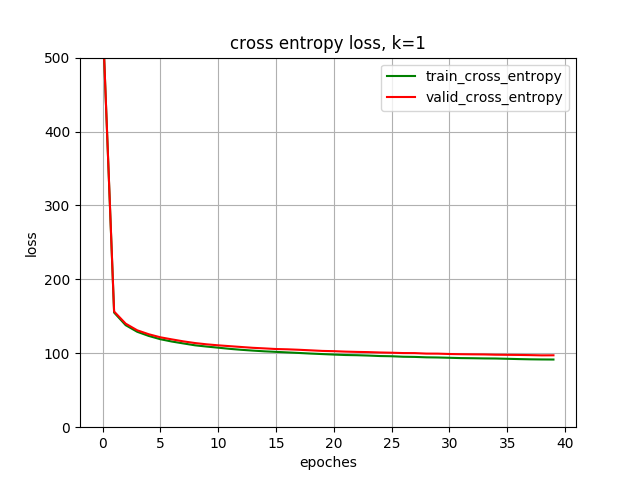
\includegraphics[width=1\textwidth]{code/cross_entropy_loss_k=1}
%loss=97.191472 
\end{minipage}
}
\subfigure[Problem a: visualization of W]{
\begin{minipage}[b]{0.4\textwidth}
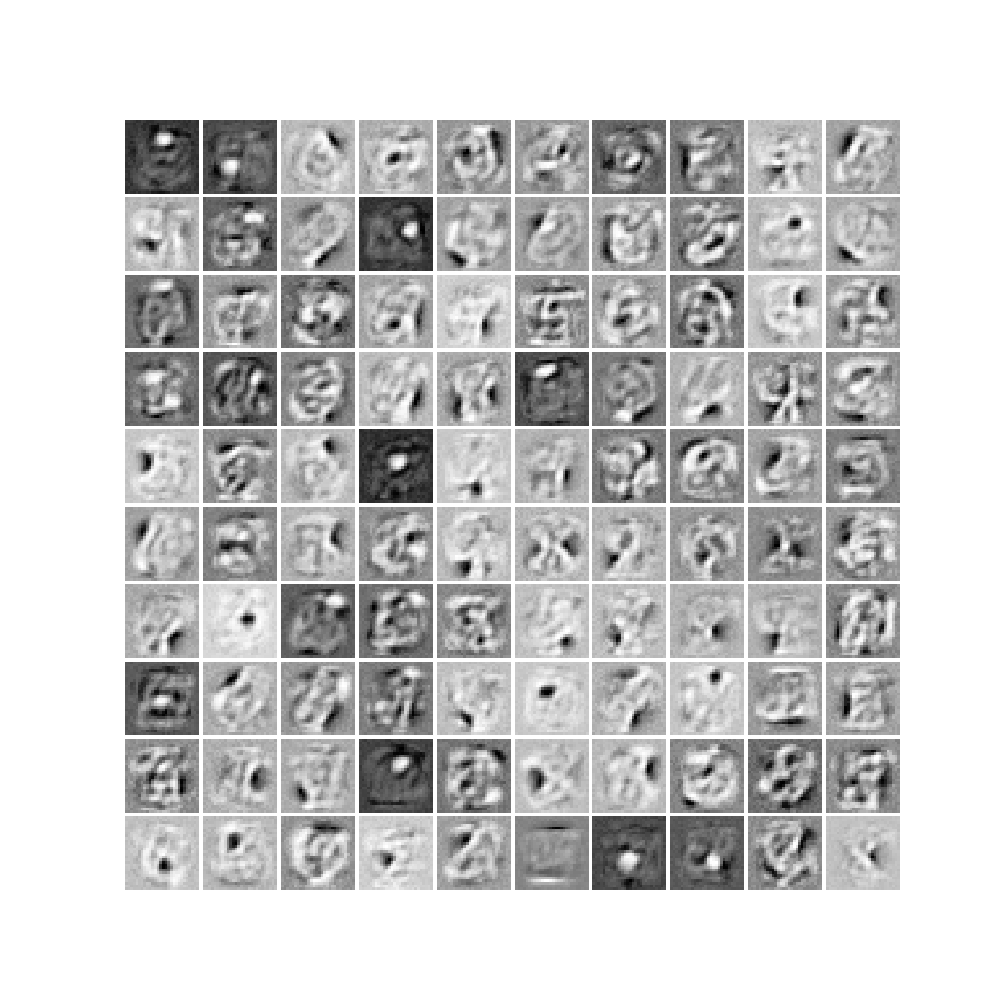
\includegraphics[width=1\textwidth]{code/k=1_W_visulization} 
\end{minipage}
}
\end{figure}
\paragraph{} In my implementation, I choose $batch\ size = 32$, $learning\ rate = 0.1$.
\paragraph{} The cross entropy loss on training set and validation set keeps decreasing without over fitting, even when I train more than 200 epochs.  The loss on training set is less than it on the validation set, and the difference is small. 
\paragraph{} The learned W has some structures and it looks like the stroke contour. 


\subsection{(b)}
\begin{figure}[h]
\centering
\subfigure[Problem b: k=5 cross entropy loss]{
\begin{minipage}[b]{0.4\textwidth}
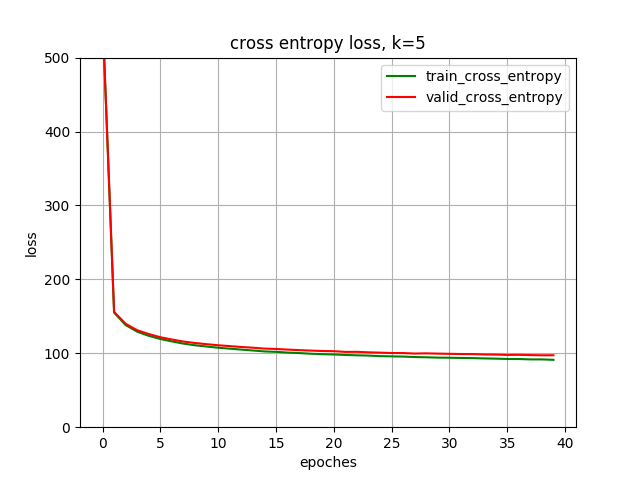
\includegraphics[width=1\textwidth]{code/cross_entropy_loss_k=5}
%_loss=97.286579 
\end{minipage}
}
\subfigure[Problem b: visualization of W]{
\begin{minipage}[b]{0.4\textwidth}
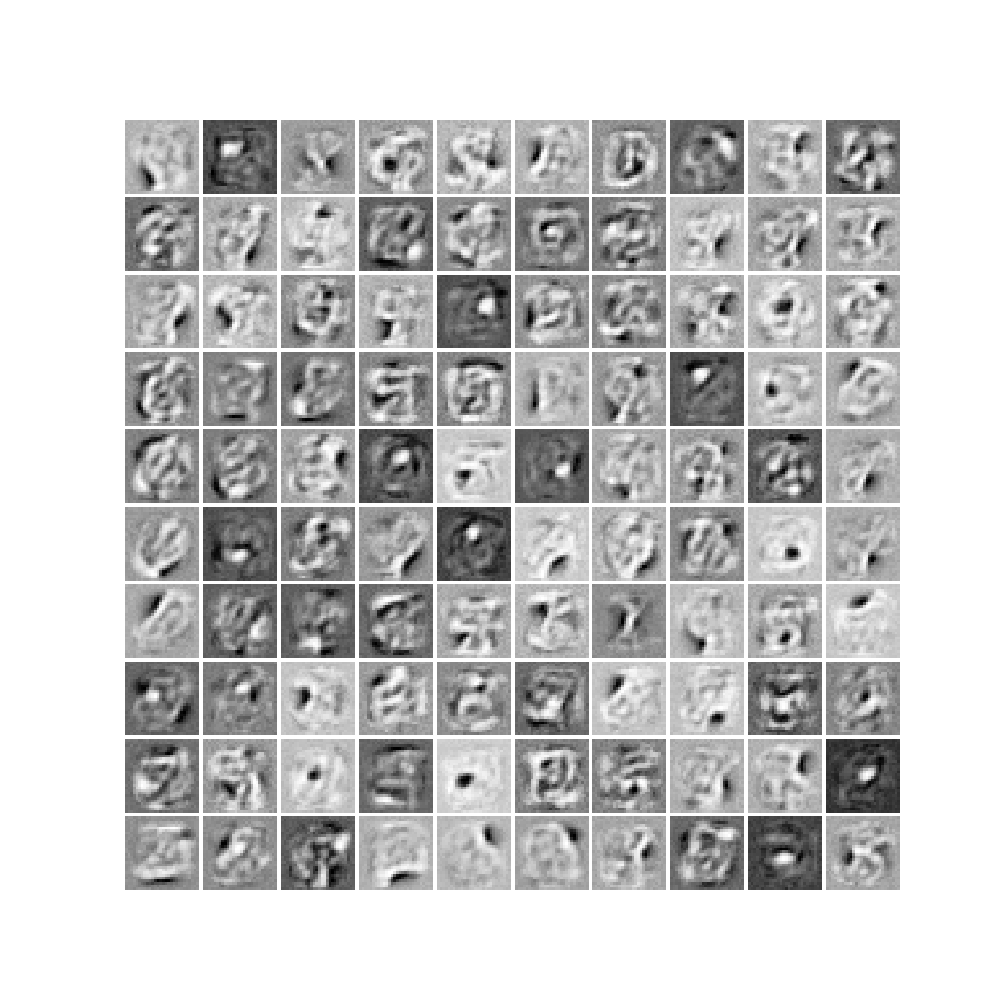
\includegraphics[width=1\textwidth]{code/k=5_W_visulization} 
\end{minipage}
}
\end{figure}

\begin{figure}[h]
\centering
\subfigure[Problem b: k=10 cross entropy loss]{
\begin{minipage}[b]{0.4\textwidth}
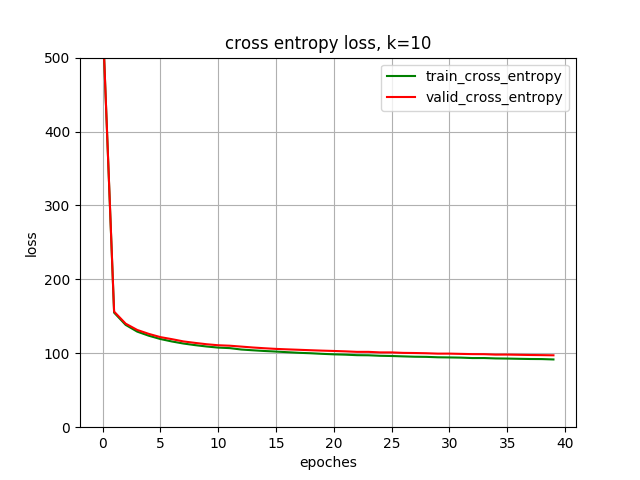
\includegraphics[width=1\textwidth]{code/cross_entropy_loss_k=10}
%_loss=97.271919
\end{minipage}
}
\subfigure[Problem b: visualization of W]{
\begin{minipage}[b]{0.4\textwidth}
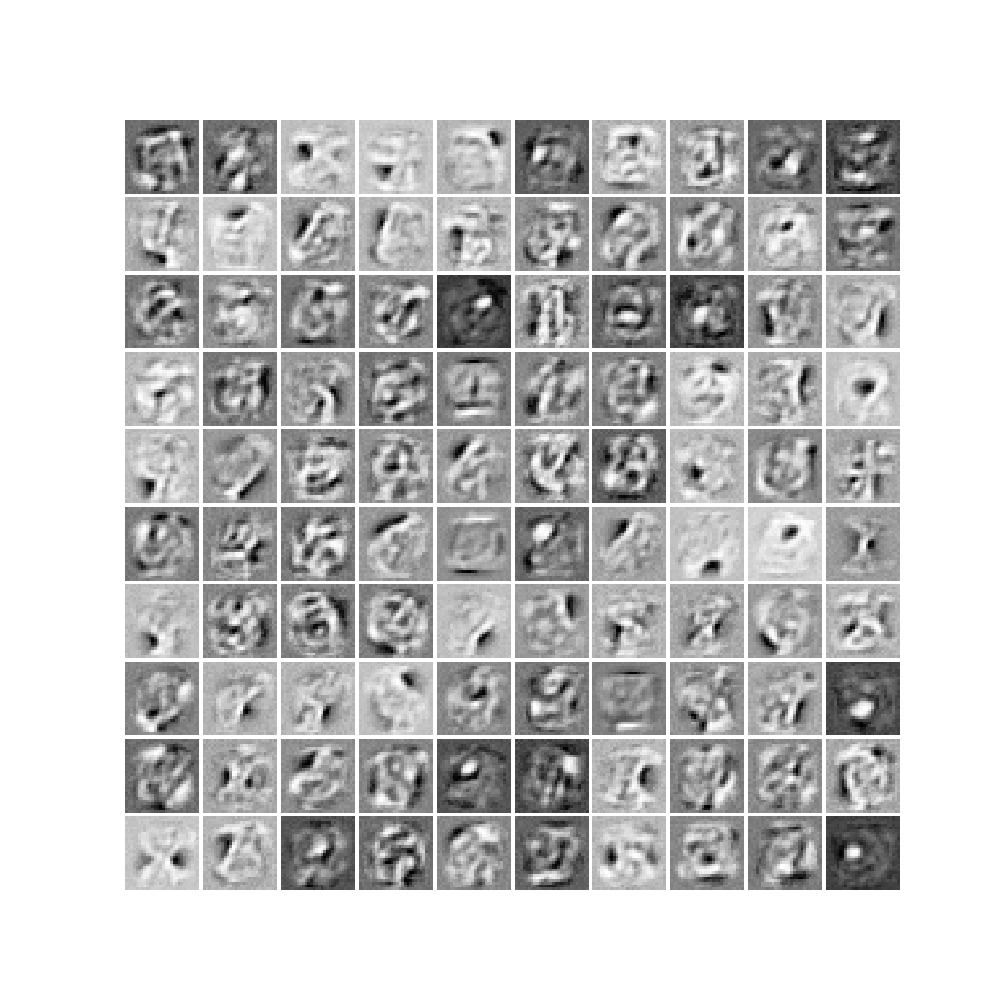
\includegraphics[width=1\textwidth]{code/k=10_W_visulization} 
\end{minipage}
}
\end{figure}

\begin{figure}[h]
\centering
\subfigure[Problem b: k=20 cross entropy loss]{
\begin{minipage}[b]{0.4\textwidth}
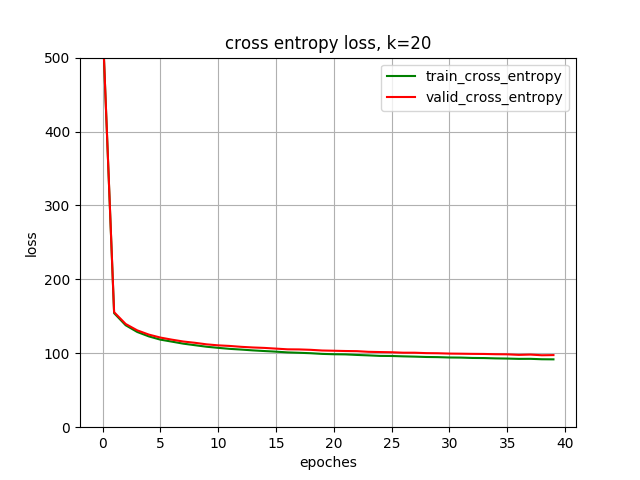
\includegraphics[width=1\textwidth]{code/cross_entropy_loss_k=20}
%_loss=97.332359 
\end{minipage}
}
\subfigure[Problem b: visualization of W]{
\begin{minipage}[b]{0.4\textwidth}
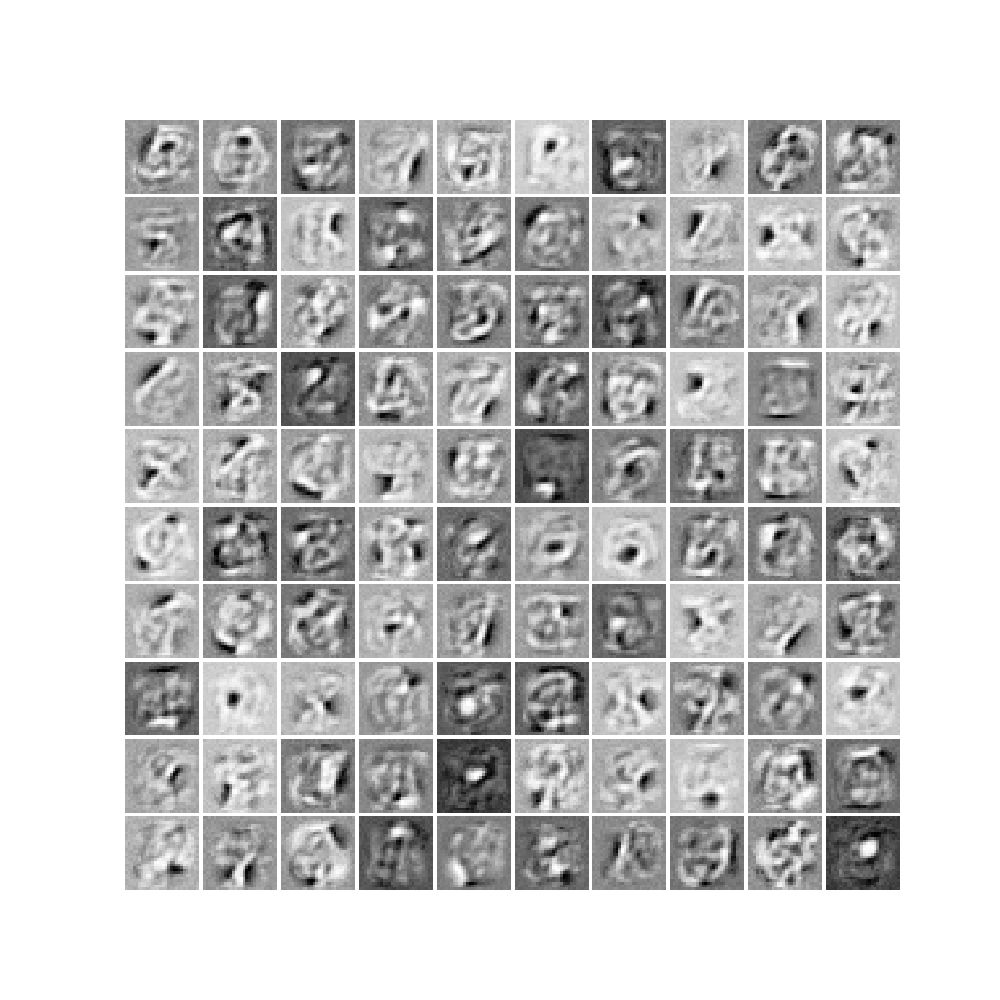
\includegraphics[width=1\textwidth]{code/k=20_W_visulization} 
\end{minipage}
}
\end{figure}
Measured by the cross entropy loss and the visualization of W, there is almost no difference between $k=1,5,10,20$. However, when I choose $k=1$, my implement can not generate reasonable images. If I choose $k \geq 5$, my implement can generate good images.

\subsection{(c)}
\begin{figure}[h]
\centering
\subfigure[Problem c: k=1 generated images]{
\begin{minipage}[b]{0.4\textwidth}
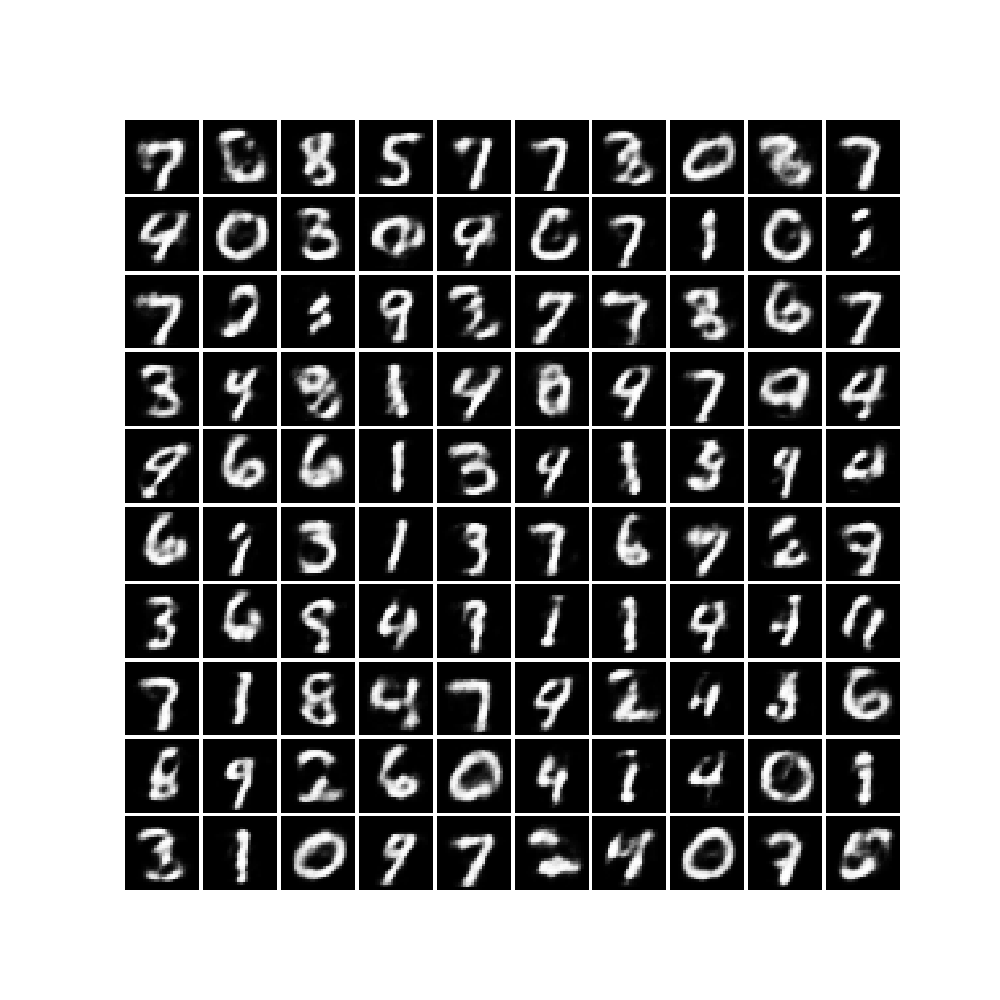
\includegraphics[width=1\textwidth]{code/generated_samples}
%_loss=97.286579 
\end{minipage}
}
\subfigure[Problem c: k=20 generated images]{
\begin{minipage}[b]{0.4\textwidth}
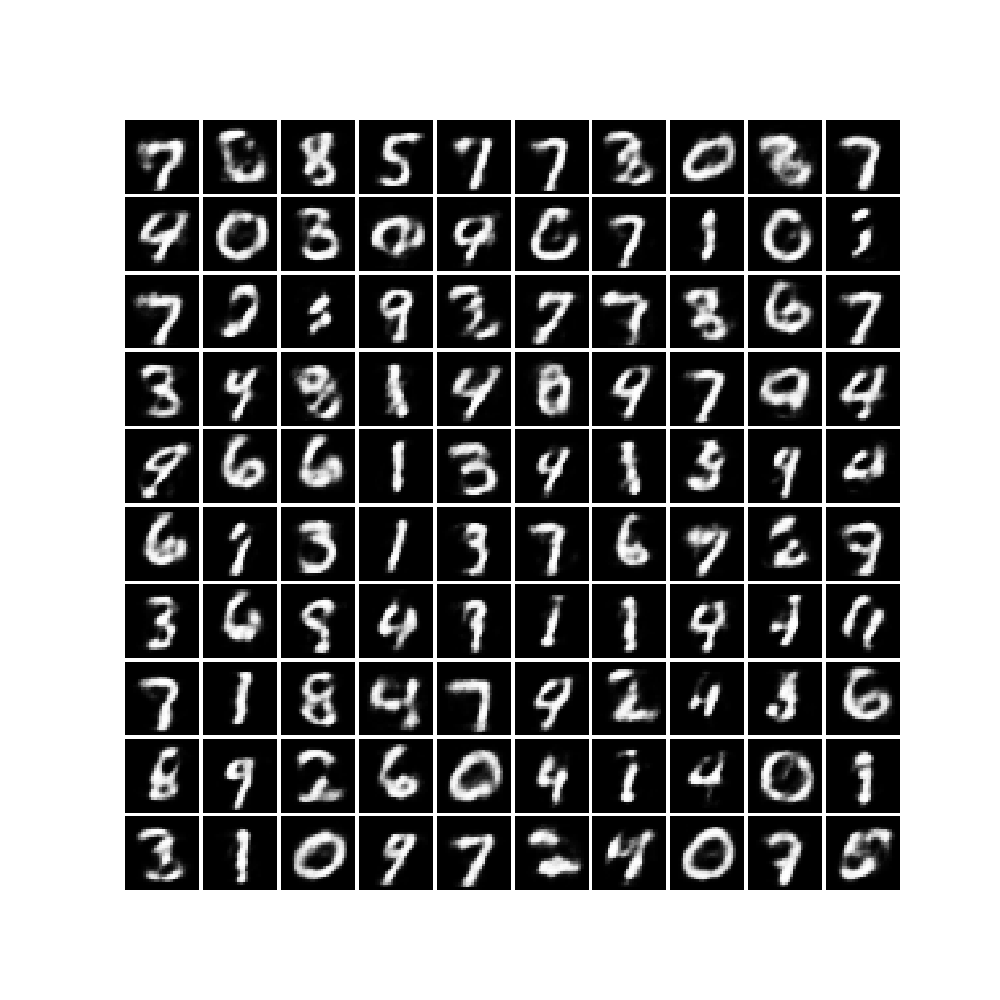
\includegraphics[width=1\textwidth]{code/generated_samples_k=20} 
\end{minipage}
}
\end{figure}
 If I choose $k \geq 5$, the generated images look like handwritten digits. The figure is the plot of $p(x|\tilde{h})$.

\subsection{(d)}
 
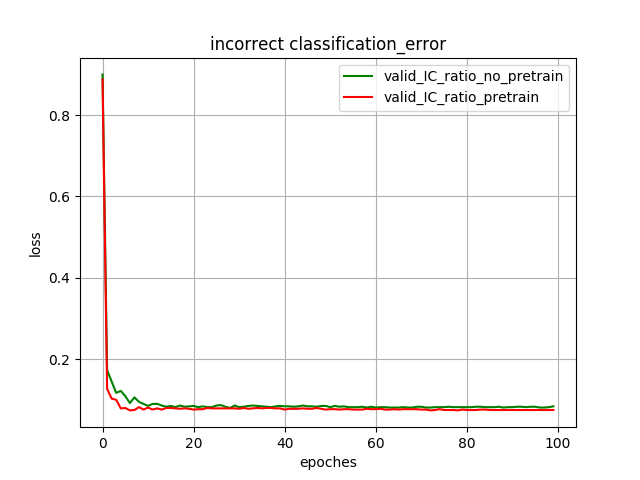
\includegraphics[width=0.5\linewidth]{code/problem_d_IC_926}
\paragraph{} After pre-training, the model converges faster, and get accuracy $92.6\%$. Without pre-training, the accuracy is $92.2\%$, which is slightly worse than the pre-training accuracy.

\subsection{(e)}

\begin{figure}[h]
\centering
\subfigure[Problem e: Pre-training accuracy vs no-pre-training accuracy]{
\begin{minipage}[b]{0.4\textwidth}
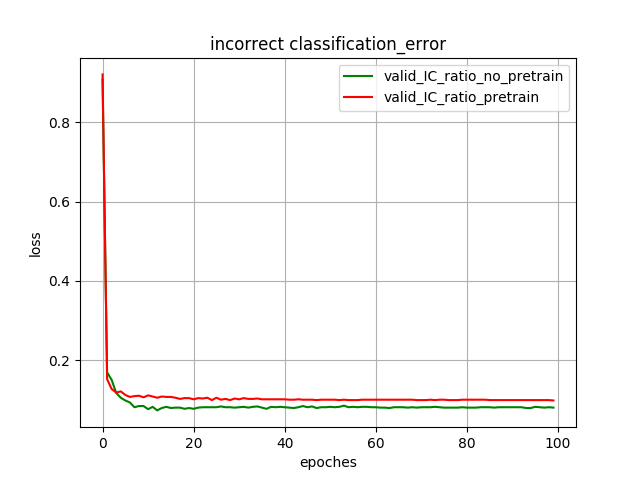
\includegraphics[width=1\textwidth]{code/Autoencoder_compare}
%_loss=97.286579 
\end{minipage}
}
\subfigure[Problem e: Visualization of W ]{
\begin{minipage}[b]{0.4\textwidth}
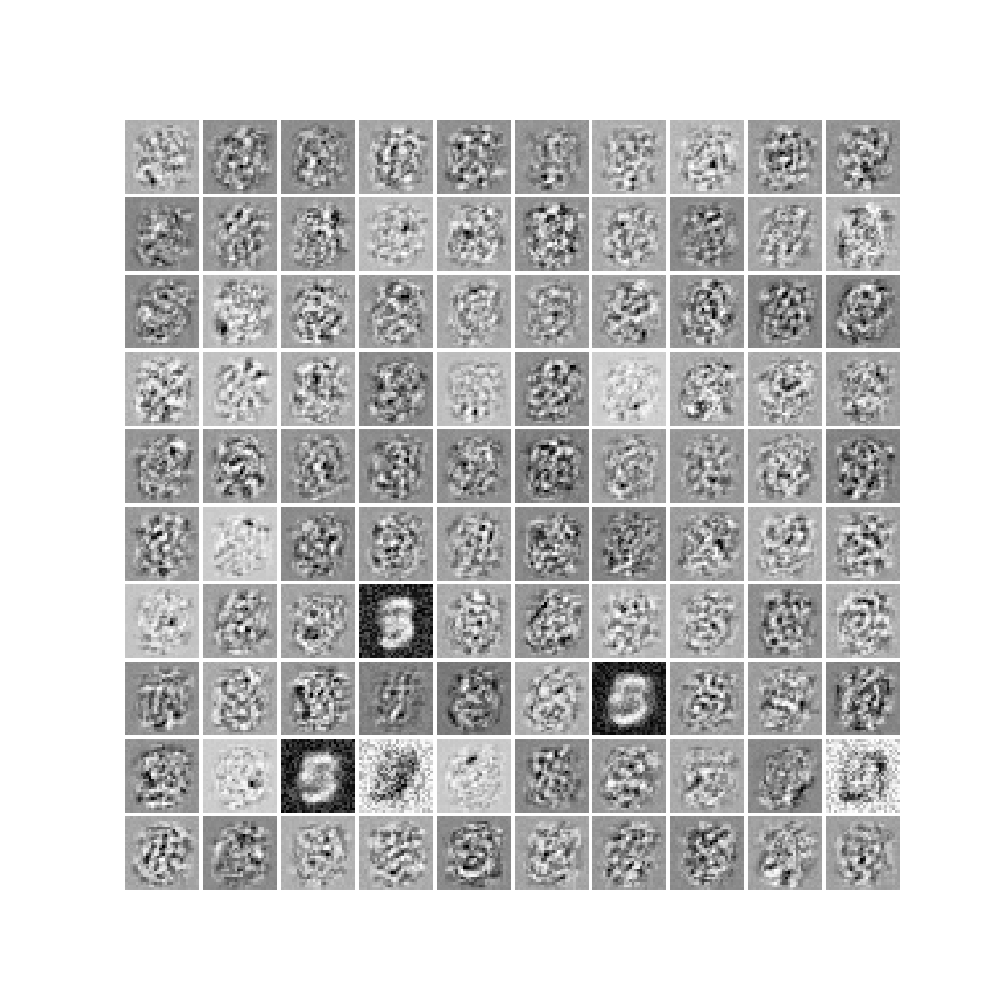
\includegraphics[width=1\textwidth]{code/Autoencoder_W_visulize} 
\end{minipage}
}
\end{figure}

\paragraph{} I use mean square error as the loss function of autoencoder, and batch size = 32. The pre-training decreases the performance, and there is almost no structure in W.

\subsection{(f)}

\begin{figure}[h]
\centering
\subfigure[Problem f: Pre-training accuracy vs no-pre-training accuracy]{
\begin{minipage}[b]{0.4\textwidth}
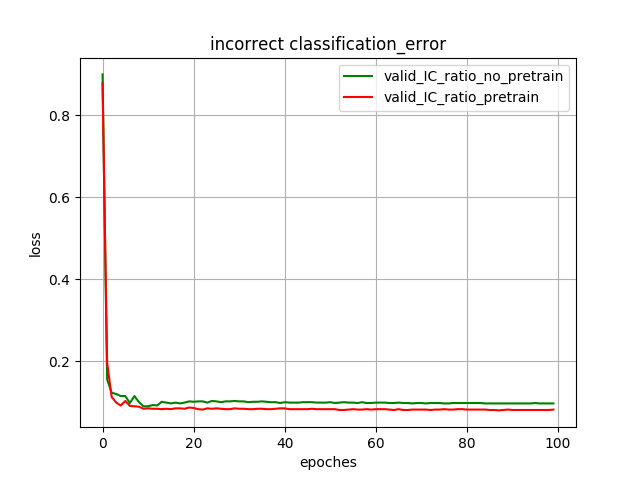
\includegraphics[width=1\textwidth]{code/Denoise_Autoencoder_compare}
%_loss=97.286579 
\end{minipage}
}
\subfigure[Problem f: Visualization of W ]{
\begin{minipage}[b]{0.4\textwidth}
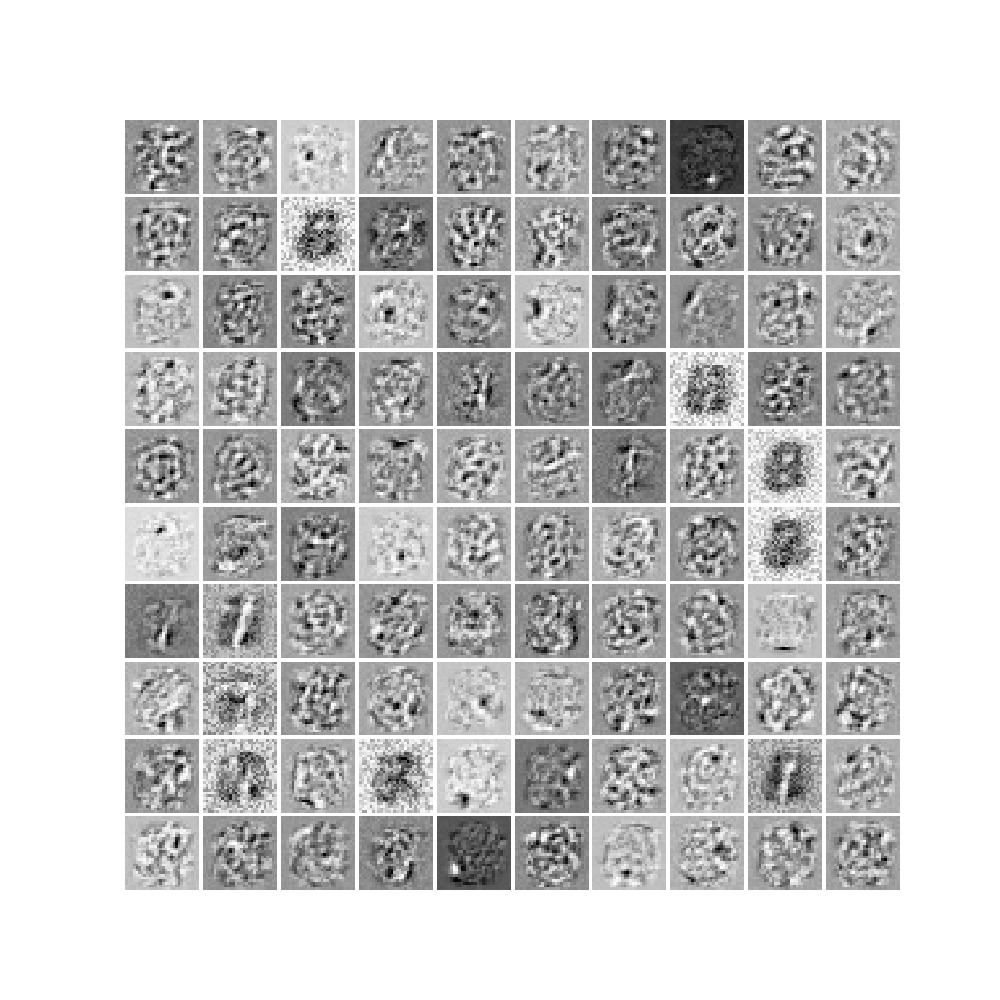
\includegraphics[width=1\textwidth]{code/Denoise_Autoencoder_W_visulize} 
\end{minipage}
}
\end{figure}

\paragraph{} In this time pre-training increases the performance slightly and the performance is almost the same as RBM pre-training. The visualization of W has some structure know. Some of the filters looks like digits: 1 and 8. 

\subsection{(g)}

\begin{figure}[h]
\centering
\subfigure[Problem g: different hidden dimension]{
\begin{minipage}[b]{0.4\textwidth}
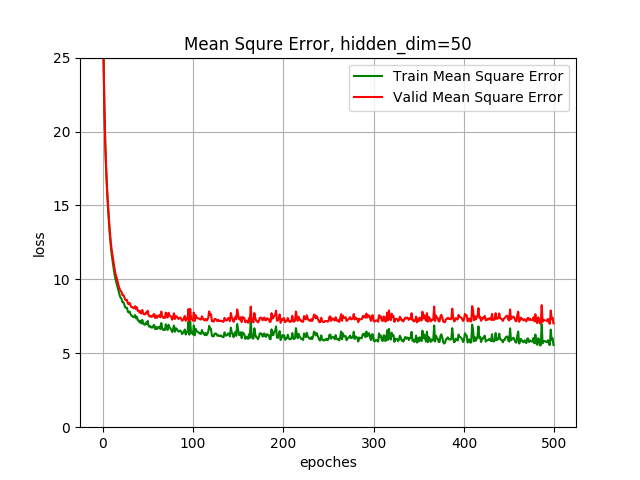
\includegraphics[width=1\textwidth]{code/problem_g_hidden50} \\
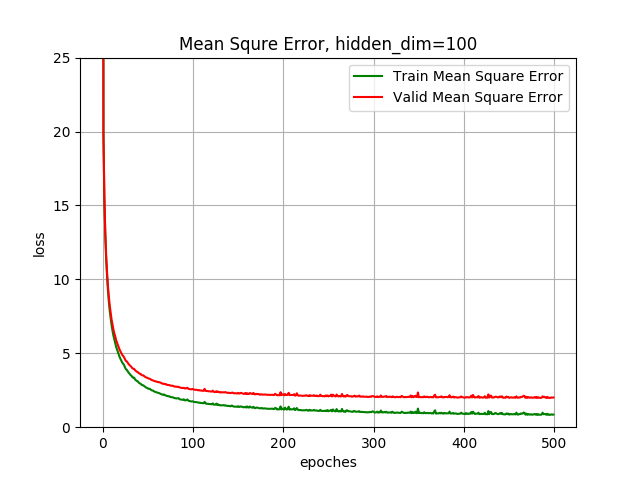
\includegraphics[width=1\textwidth]{code/problem_g_hidden100}
\end{minipage}
}
\subfigure[Problem d: different momentum]{
\begin{minipage}[b]{0.4\textwidth}
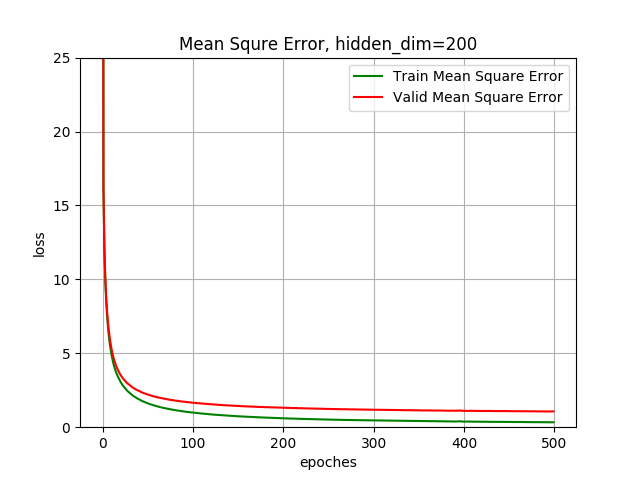
\includegraphics[width=1\textwidth]{code/problem_g_hidden200} \\
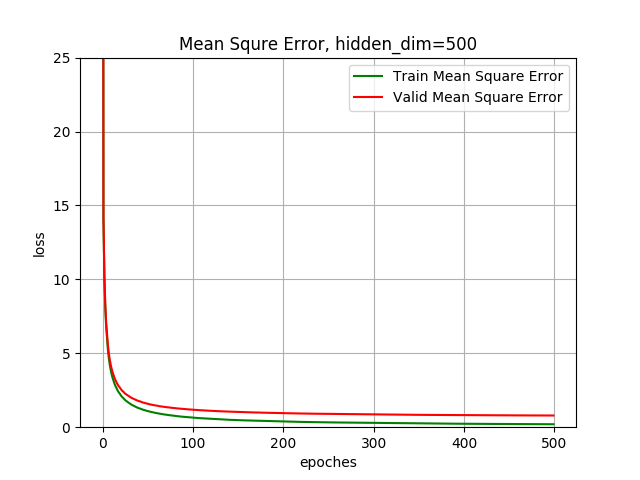
\includegraphics[width=1\textwidth]{code/problem_g_hidden500}
\end{minipage}
}
\end{figure}
\paragraph{} With the increasing of hidden dimension, the loss will decrease a lot, and the loss curve will become more and more smooth.
\end{document}

\grid